\chapter{REFERENCIAL TEÓRICO}

Nesta seção, será descrita a base teórica da pesquisa aqui desenvolvida.


\section{INTELIGÊNCIA ARTIFICIAL}

A inteligência artificial é o estudo de agentes que recebem percepções do ambiente e realizam ações. Um agente opera autonomamente, percebe seu ambiente e persiste por um longo período de tempo, adaptando-se a mudanças e perseguindo seu objetivo \cite{russell2003ai}.

\begin{figure}[H]
    \centering
    \caption{Campos de estudo de Inteligência Artifial.}
    \label{fig:conjunto-ia}
    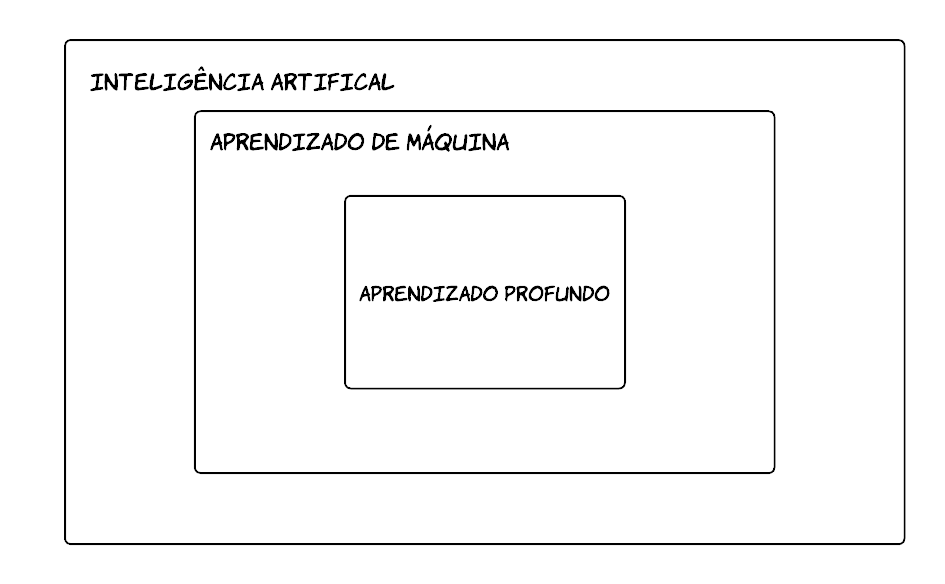
\includegraphics[width=0.9\textwidth]{imagens/conjunto-ia-ml-dl-PTBR.png}


    
    {\footnotesize \textbf{Fonte:} A Autora (2026).}
\end{figure}


\subsection{Aprendizado de Máquina}

 O ciclo descrito é mostrado na figura abaixo:

\begin{figure}[htbp]
    \centering
    \caption{Fluxograma da construção de um algoritmo de aprendizado de máquina.}
    \label{fluxograma-ai-ml}

    % 1. Definimos a caixa de ícone FORA do tikzpicture
    \newcommand{\iconbox}[1]{%
        \tikz[baseline=-0.5ex]{%
            \node[fill=white, text=black, rounded corners=2pt, inner sep=4pt, minimum height=0pt, minimum width=0pt, text width=]{\Large #1};%
        }\\[0.2cm]%
    }

    % 2. AJUSTE AQUI: Mudamos de \textwidth para 0.8\textwidth (80% do tamanho da linha)
    \resizebox{0.7\textwidth}{!}{%
    \begin{tikzpicture}[
        % Espaçamento global entre os nós
        node distance=1.5cm and 1cm,
        % Estilo base para todos os nós
        base/.style={
            fill=white,         % Alterado de 'mygreen' para branco
            draw=black,         % Mantém a borda preta
            text=black,         % Garante o texto em preto
            font=\sffamily\bfseries\small, 
            text width=4.2cm, 
            align=center, 
            minimum height=2.8cm, 
            inner sep=0.3cm
        },
        % Estilo para as caixas retangulares
        box/.style={
            base,
            rectangle, 
            rounded corners=4pt
        },
        % Estilo para a caixa inicial (formato de pílula)
        oval/.style={
            base,
            rectangle,
            rounded corners=1.4cm
        },
        % Estilo das setas
        arrow/.style={
            ->, 
            =latex, 
            draw=black!70,
            thick
        }
    ]

    % ==================== NÓS DO FLUXOGRAMA ====================
    \node (n1) [oval] {\iconbox{\faDatabase}1 - COLETA DE DADOS\\(DADOS BRUTOS)};

    \node (n2) [box, right=of n1] {\iconbox{\faCogs}2 - PROCESSAMENTO PARA NORMALIZAÇÃO E PADRONIZAÇÃO DOS DADOS};

    \node (n3) [box, right=of n2] {\iconbox{\faRobot}3 - TREINAMENTO DO MODELO};

    % Posicionando a segunda linha de nós
    \node (n4) [box, below=2cm of n3] {\iconbox{\faChartLine}4 - APLICAÇÃO EM CENÁRIO REAL};

    \node (n5) [box, left=of n4] {\iconbox{\faBrain}5 - TOMADA DE DECISÃO INTELIGENTE PELO ALGORITMO DE ML};

    % ==================== SETAS DE CONEXÃO ====================
    \draw [arrow] (n1) -- (n2);
    \draw [arrow] (n2) -- (n3);

    % Seta do N3 para o N4 
    \draw [arrow] (n3.south) -- ++(0,-0.8) -| ([xshift=0.8cm]n4.east) -- (n4.east);

    % Seta do N4 para o N5
    \draw [arrow] (n4) -- (n5);

    \end{tikzpicture}%
    }

    \vspace{0.4cm}
    {\footnotesize \textbf{Fonte:} Feitosa; Santos; Sousa (2023).}
\end{figure}

\vspace{2.0cm}




\section{CRIPTOGRAFIA}

Para entender o que é a criptografia, é necessário antes inteirar-se de alguns conceitos-base. Texto claro é a mensagem original, legível. Texto cifrado é quando a mensagem original é codificada. O processo de transformar um texto claro em um texto cifrado é chamado de \textbf{cifração}; converter um texto cifrado em um texto claro novamente é denominado \textbf{decifração}.

\begin{table}[H]
    \centering
    \caption{Conceitos base da criptografia.}
    \label{conceitos_cripto}

    \begin{tabular}{|p{4cm}|p{10cm}|}
        \hline
        \rowcolor[HTML]{EFEFEF} 
        \multicolumn{1}{|c|}{\textbf{Conceito Base}} & \multicolumn{1}{c|}{\textbf{Definição}} \\ \hline
        Texto Claro & Mensagem que deve ser protegida, denominada \textit{M}. \\ \hline
        Texto Cifrado & Mensagem cifrada, denominada \textit{C}. \\ \hline
        Chave & Valor numérico utilizado por um algoritmo para cifrar uma mensagem, fazendo com que a mensagem original seja recuperável mediante utilização deste valor. \\ \hline
        Cifração & Método utilizado para transformar uma mensagem \textit{M}. Sendo \textit{E} uma função de cifração e \textit{k} uma chave, então cifrar pode ser definido como $E_k(M) = C$. \\ \hline
        Decifração & Método para recuperar a mensagem original. Sendo \textit{D} uma função de decifração e \textit{k} uma chave, então decifrar pode ser definido como $D_k(C) = M$. \\ \hline
    \end{tabular}

    \vspace{0.4cm}
    {\footnotesize \textbf{Fonte:} A Autora (2026).}
\end{table}




\subsection{A Criptogrfia Simétrica - Chave Secreta Compartilhada}


A PKC depende das chamadas \textit{trapdoor functions}: são funções matemáticas que são simples de se calcular, ao passo que,  suas funções matemáticas inversa possuem um grau de complexidade matemática . Para explicar tal lógica vamos utilizar como exemplo a potenciação abaixo:

\begin{equation}
   3^6 = 759 
  \label{eq:cifra_publica_funcao}
\end{equation}










